\section{Chapters and Referenced Files}
\label{sec:files}

The converter is given a directory.
It may be a folder that contains only the chapters, or a whole repository with a README, several
documentation folders, and an archive of old notes, any of which may contain Markdown files.
Before anything is rendered, the converter must decide which files become chapters, in which order,
and under which titles.
It must also determine how referenced files get into the package.

\subsection{Chapter Folder, Order, and Titles}
\label{sec:in_folder}

\paragraph{Locating the Chapter Folder.}
In a repository, the chapters are rarely at the root.
A repository typically holds a README at the top, the chapters somewhere below it, and often other
folders with Markdown files that are not part of the book.
Instead of requiring the user to always name the folder, the converter locates it on its own.
It reports which other folders it could have chosen, so that the user can convert again with an
explicit choice if the guess was wrong.

\begin{figure}[H]
	\centering
	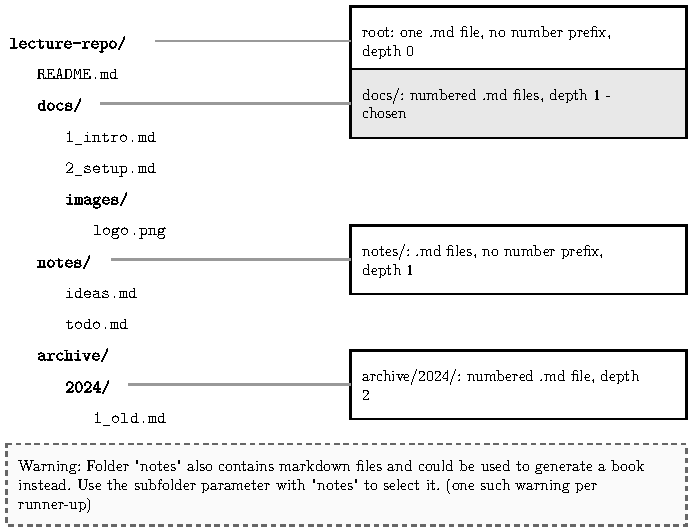
\includegraphics[width=0.9\columnwidth]{figures/chapter-folder}
	\caption[Locating the chapter folder]{\label{fig:chapter_folder}Locating the chapter folder in a repository with four
		folders that directly contain Markdown.
		The root and \code{notes/}
		have no numbered file; \code{archive/2024/} has one but lies deeper than
		\code{docs/}, which is chosen.
		Each runner-up produces one warning naming the
		parameter that would select it instead.}
\end{figure}

Only folders that contain Markdown files are candidates.
Among them, the converter prefers
a folder containing a Markdown file with a leading number in its name, since this is
the chapter-ordering convention described below;
the shallowest folder, since archives and drafts tend to lie deeper than the chapters;
and, on a tie, the alphabetically first.
Every candidate not chosen is named in a warning, together with the subfolder parameter
that would select it.
\autoref{fig:chapter_folder} shows a repository with four candidates and the resulting choice.
Alternatively, an explicit subfolder parameter skips the search.
It must lie within the input directory; if it does not exist, the search still runs, and a
warning is issued.

\paragraph{Chapter Order.}
\label{sec:in_order}
Inside the chosen folder, every file with the extension \code{.md} becomes a chapter.
Subfolders are not searched, so that a folder of images or appendices next to the chapters does not
add chapters.
Files whose name starts with a digit come first, sorted by the numeric (rather than alphabetic) value of that prefix,
so \code{10\_summary.md} follows \code{2\_setup.md}.
Files without a number follow in alphabetical order.
If a folder mixes the two conventions, a warning names the unnumbered files, but none of them is
dropped, since silently dropping a chapter would lose content.
The number prefix may be followed by a dot, a parenthesis, a hyphen, an underscore, or spaces, all of
which are stripped.

\paragraph{Chapter Titles.}
The title of a chapter is the text of its first heading, if the file starts with one.
YAML front matter at the top of the file does not count as content, so a heading right after it
still counts as first.
Otherwise, the title is the file name without the number prefix and with underscores replaced by
spaces, so \code{3\_getting\_started.md} becomes ``getting started''.
A heading that became the title is also kept in the chapter body.
The sidebar entry that shows the title is often truncated, and a chapter that opens without a
visible heading reads worse than one whose title appears twice.

\subsection{Path Resolution and Trust Boundaries}
\label{sec:files_paths}


In practice, the files referenced by a chapter are images, and every reference is a path that the converter has to resolve to a file.
Unlike chapter discovery, path resolution depends on the input mode, because a path can point anywhere.
A Markdown file containing \code{![](../../../etc/}\allowbreak\code{passwd)} makes no sense as documentation.
A server that resolves this path and packs the file into a downloadable archive, however, leaks a
file from its own disk to whoever submitted the repository.
This is the path traversal weakness cataloged as CWE-22~\cite{MITRE:CWE22}, which the converter has
to prevent on the server without breaking the normal case on the desktop.

\paragraph{Trust Boundaries.}
A clone or an upload was written by somebody other than the operator, so its content must not
reach anything outside the directory it was placed in.
A local folder, by contrast, is converted by the person running the command, who already has full access to the
file system.
Restricting it would protect nobody and would break notes that reference an image elsewhere on the
disk, for instance in a shared assets folder or on another drive.
The policy therefore depends on the input mode: a local folder is unrestricted, while a clone or an
upload is confined to its directory.
The same trust boundary applies to downloading remote images.

\paragraph{Resolution Order.}
A referenced path is resolved in four steps.
\circled{1} It is interpreted relative to the directory of the Markdown file that contains it, and
if a file exists there, that file is used.
\circled{2} Otherwise, it is interpreted as an absolute path.
The relative interpretation comes first because a repository-style path such as
\code{/images/logo.png} would otherwise be read as absolute on Unix systems and fail.
\circled{3} The result is canonicalized, applying every \code{..} and resolving symbolic links,
so that the following check cannot be bypassed.
\circled{4} For a clone or an upload, the canonical path has to lie inside the input directory;
otherwise the reference is rejected.
A rejected path, a nonexistent file, and a path that cannot be canonicalized at all
each produce a warning; the image is omitted.

\paragraph{Uploads and Submitted Packages.}
Two further kinds of names come from outside and are checked in the same way.
In a multipart upload, the client names every file, and a name such as \code{../../x.md} would
otherwise place the file outside the staging directory. Such a file is rejected.
A package submitted for merging is a ZIP archive whose entry names are chosen
by the client as well, and an entry that is absolute or leaves its directory is rejected for the same
reason.
The merge reads the archive without unpacking it, which avoids most of this problem in the first
place.

\subsection{Images}
\label{sec:sec_images}

Images are referenced in nearly every chapter. They have to be copied into the package because
H5P has no notion of an image stored elsewhere.
This raises three questions: what an image is called inside the package, which files may be
included, and how to handle images that are not local files.

\paragraph{Naming in a Flat Folder.}
All images of a book end up in the single folder \code{content/images} of the package, regardless of
how the author's folders were organized.
The file name alone is not unique: two chapters that both reference a file named
\code{logo.png} in different folders would map onto the same entry, and a duplicate entry would abort the creation of the
archive.
The converter therefore appends the first twelve bytes of the image's SHA-256 hash to its sanitized file name,
followed by the extension, for instance \code{logo-3f9a2c17b0e4d5a6c1f83a23.png}.
Collisions between different files are thus extremely unlikely, and repeated references to the same
image share a single stored copy.
Moreover, the packed name does not depend on where the file was located on the author's machine.


\paragraph{Accepted Formats.}
Moodle validates every file in a package against a list of allowed extensions, and a package with a
single file outside that list is rejected as a
whole\footnote{\raggedright \code{validateContentFiles} in \code{h5p.classes.php}, lines 4420--4454, against
the list \code{H5PCore::\$defaultContentWhitelist} at line 2118; Moodle passes the list through
unchanged (\code{h5p/classes/framework.php}, line 698).}~\cite{H5P:PhpLibrary}.
For images, the list contains \code{png}, \code{jpg}, \code{jpeg}, \code{gif}, \code{bmp},
\code{tif}, and \code{tiff}.
Any other image, such as \code{webp}, \code{svg}, or a file with no extension, is therefore omitted from the
package with a warning.
If it were included, Moodle would reject the entire book.
Only the extension is checked, not the file content. Unsupported formats are not converted,
since this would add an image-processing dependency for a problem that belongs in the source
document.
In practice, \code{svg} is the most common case, because diagrams are often kept in that format;
the author has to export them as PNG.

\paragraph{Remote Images.}
Markdown allows an image to be referenced by URL, which is common in notes written in a wiki or an
issue tracker.
Since the package cannot reference anything outside itself, the converter downloads the image at
conversion time and treats it like a local file, with the same extension check and naming.
Leaving the reference in the markup is not an option, because the sanitizer removes every
\code{img} tag and only the alternative text would remain.
A reference counts as remote if it starts with a scheme of at least two letters, so that a Windows
path such as \code{C:/notes/logo.png} is not mistaken for a URL.
The content type of the response is checked as well, so that an HTML error page returned with
status 200 is not packed as an image.
If the URL has no extension, that same content type determines the file type.

On the web server, the download is a request to an address chosen by a stranger.
A request to \code{http://127.0.0.1:8080/} or to a cloud provider's metadata endpoint would be made
from inside the server, and the response would be packed into a book anyone can download.
This is known as server-side request forgery.
The download is therefore limited in four ways:
a timeout;
a size limit of 20 MB, enforced while reading instead of relying on the \code{Content-Length}
header;
a refusal of any loopback, link-local, site-local, unique-local, or multicast address;
and redirects, at most three, checked as well since the target of a redirect may also be a private
address.
As with paths, the address check applies to a clone or an upload but not to a local folder.
Somebody converting their own notes can open these addresses in a browser anyway, and notes that
reference a wiki or a documentation server on \code{localhost} are a legitimate case.

\paragraph{Embedded Images.}
A \code{data:} URL contains the image itself, base64- or percent-encoded, and some Markdown editors
write one when an image is pasted into a document.
Such a URL is decoded instead of downloaded, its media type takes the role of the content type, and
the result is treated like a local file.

Every failure described in this section produces a warning, but the book is still produced.
